\documentclass[a4paper,12pt]{article}
\usepackage{amsmath}
\usepackage{amssymb}
\usepackage[polish]{babel}
\usepackage{polski}
\usepackage[utf8]{inputenc}
\usepackage{indentfirst}
\usepackage{geometry}
\usepackage{array}
\usepackage[pdftex]{color,graphicx}
\usepackage{subfigure}
\usepackage{afterpage}
\usepackage{setspace}
\usepackage{color}
\usepackage{wrapfig}
\usepackage{listings}
\usepackage{datetime}
\usepackage{float}

\title{PRiR Zadanie 3}
\renewcommand{\onehalfspacing}{\setstretch{1.6}}

\geometry{tmargin=2.5cm,bmargin=2.5cm,lmargin=2.5cm,rmargin=2.5cm}
\setlength{\parindent}{1cm}
\setlength{\parskip}{0mm}

\newenvironment{lista}{
\begin{itemize}
  \setlength{\itemsep}{1pt}
  \setlength{\parskip}{0pt}
  \setlength{\parsep}{0pt}
}{\end{itemize}}

\newcommand{\linia}{\rule{\linewidth}{0.4mm}}

\definecolor{lbcolor}{rgb}{0.95,0.95,0.95}
\lstset{
    backgroundcolor=\color{lbcolor},
    tabsize=4,
  language=C++,
  captionpos=b,
  tabsize=3,
  frame=lines,
  numbers=left,
  numberstyle=\tiny,
  numbersep=5pt,
  breaklines=true,
  showstringspaces=false,
  basicstyle=\footnotesize,
  identifierstyle=\color{magenta},
  keywordstyle=\color[rgb]{0,0,1},
  commentstyle=\color{Darkgreen},
  stringstyle=\color{red}
  }

\begin{document}

\noindent
\begin{tabular}{|c|p{11cm}|c|} \hline 
Grupa 3 & Albert Soczewski, Maciej Ząbek & \ddmmyyyydate\today \tabularnewline
\hline 
\end{tabular}


\section*{Zadanie 3 - Rozmycie Gaussa w CUDA}

Celem zadania było wykonanie programu rozmywającego zadane zdjęcie za pomocą
algorytmu Gaussa z maską o wymiarach 5x5. Do zrównoleglenia operacji wykorzystana została technologia CUDA, natomiast funkcjonalości potrzebne do pracy z obrazami zapewnione zostały dzięki bibliotece OpenCV.

Do rozmycia została użyta maska o poniższych wartościach:
\begin{figure}[ht]
\centering
\begin{tabular}{|l|l|l|l|l|}
\hline
0 & 1 & 2 & 1 & 0 \\ \hline
1 & 4 & 8 & 4 & 1 \\ \hline
2 & 8 & 16 & 8 & 2 \\ \hline
1 & 4 & 8 & 4 & 1 \\ \hline
0 & 1 & 2 & 1 & 0 \\ \hline
\end{tabular}
\caption{Zastosowany filtr wykorzystujący funkcje Gaussa}
\end{figure}

Dla wczytanego obrazu zostaje dodana ramka o rozmiarze 2 pikseli, które są kopiami pikseli brzegowych. Ma to na celu ułatwienie zastosowania maski dla pikseli na krawędziach obrazka.

Algorytm rozmycia został zaimplementowany podobnie jak w poprzednim zadaniu:
\begin{lstlisting}
__global__ void gaussianBlur(uchar * inputImage, uchar * outputImage, long width, long height)
{
    long x = (blockIdx.x * blockDim.x) + threadIdx.x;
    long y = (blockIdx.y * blockDim.y) + threadIdx.y;

    if (x < width-2 && y < height-2 && x>1 && y>1)
    {
        long r=0, g=0, b=0;
        long pixelIn, pixelOut;

        for (int y_m = 0; y_m<5; y_m++)
        {
            for (int x_m = 0; x_m<5; x_m++)
            {
                pixelIn = width*(y + y_m - 2) * 3 + (x + x_m - 2) * 3;

                r += inputImage[pixelIn + 2] * dev_mask[x_m][y_m];
                g += inputImage[pixelIn + 1] * dev_mask[x_m][y_m];
                b += inputImage[pixelIn] * dev_mask[x_m][y_m];
            }
        }
        pixelOut = (width - 4)*(y - 2) * 3 + (x - 2) * 3;
        outputImage[pixelOut + 2] = r / dev_weight;
        outputImage[pixelOut + 1] = g / dev_weight;
        outputImage[pixelOut] = b / dev_weight;
    }
}
\end{lstlisting}

Algorytm dla każdego piksela (z pominięciem ramki) pobiera wartości kolorów składowych, wyznacza nową wartość piksela (na podstawie otaczających go sąsiadów) oraz dokonuje zapisu na nowym obrazie. \newline

\noindent W celu uzyskania odpowiednich rezultatów, do wczytanego obrazu dodana zostaje ramka złożona z kopii pikseli brzegowych. 

\begin{lstlisting}
 copyMakeBorder(inputImage, inputImage, 2, 2, 2, 2, BORDER_REPLICATE);
\end{lstlisting}

Stosując się do wskazówek autorów książki 'CUDA w przykładach' wybraliśmy rozwiązanie problemu polegające na podzieleniu obrazu na tyle wątków z ilu składa się pikseli. W tym celu zdefiniowaliśmy najpierw dwie dwuwymiarowe zmienne o nazwach gridSize oraz threadsPerBlock. Pierwsza reprezentuje liczbę bloków, a druga - liczbę wątków na blok. Dzięki temu każdy wątek posiada unikalny indeks (x,y) dzięki któremu jest możemy powiązać go z pixelem w obrazie wejsciowym. Po przeprowadzeniu testów uznaliśmy, że najbardziej optymalny rozmiar bloku wynosi 32 x 32(1024 wątki per blok). Aby przy takim rozmiarze bloku otrzymać po jednym wątku na piksel należy uruchomić odpowiednią ilość bloków. Cały proces przedstawiony jest na listingu poniżej.

\begin{lstlisting}
	int gridWidth, gridHeight;
    gridWidth = inputImage.cols / blockSize + ((inputImage.cols % blockSize) == 0 ? 0 : 1);
    gridHeight = inputImage.rows / blockSize + ((inputImage.rows % blockSize) == 0 ? 0 : 1);

    dim3 gridSize(gridWidth, gridHeight);
    dim3 threadsPerBlock(blockSize, blockSize);
\end{lstlisting}

Po deklaracjach zmiennych do przechowywania wymiarów uruchamiamy jądro które będzie obliczało wartości pikseli po zastosowaniu rozmycia Gaussa.

\begin{lstlisting}
    gaussianBlur <<< gridSize,threadsPerBlock >>> (dev_inputImage, dev_outputImage, inputImage.cols, inputImage.rows);
\end{lstlisting}

Poniższy wykres przedstawia zależność czasu wykonywania programu od liczby wątków w bloku. Badany obraz miał wymiary 4032x2268px. Zrównoleglenie zostało wykonane dla rozmiaru bloku od 1 do 32. Wynika to z faktu, że maksymalna liczba wątków w bloku to 1024 (32x32), dlatego w celu znalezienia optymalnej liczby przebadaliśmy wszystkie możliwe konfiguracje siatki oraz liczby wątków w bloku zachowując sumaryczną ilość wątków równą liczbie pikseli w obrazie.

\begin{figure}[H]
	\centering
  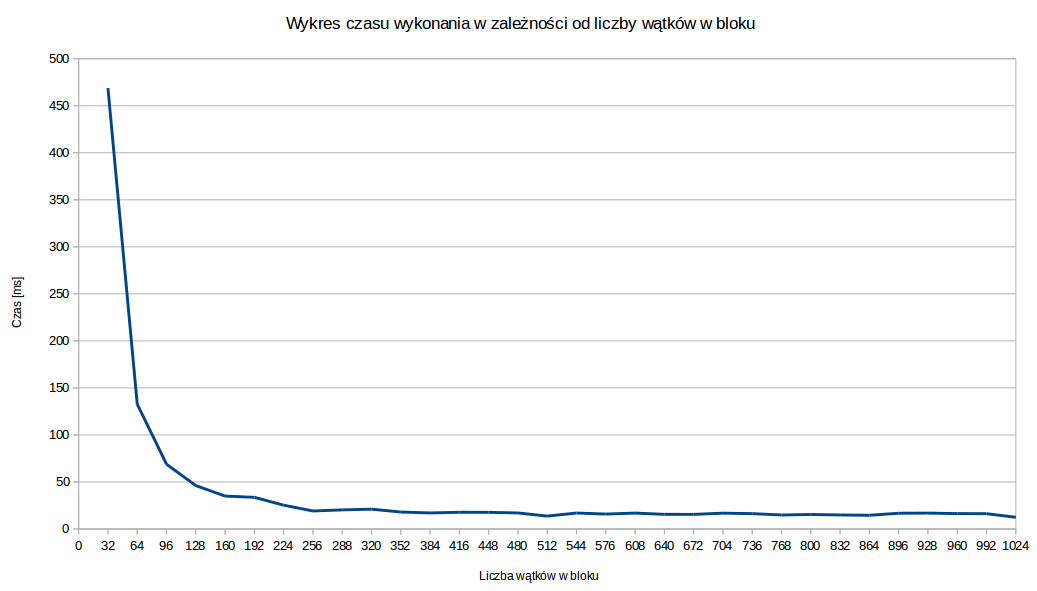
\includegraphics[width=0.75\textwidth]{dane/wykres1.png}
  \caption{Wykres czasu wykonania w zależności od liczby wątków w bloku}
\end{figure}

Na wykresie można zaobserwować, że w czas wykonania malał gdy liczba wątków się zwiększała. Największy zysk jest zauważalny do uruchomienia około 256 wątków per blok. Po osiągnięciu tego progu czas ustabilizował się. Najmniejszy czas operacji zanotowano dla 1024 wątków.

Zadanie zostało zrealizowane, a otrzymane wyniki są zadowalające.
Zrównoleglając operacje przy technologii CUDA udało się uzyskać satysfakcjonującą poprawe czasu wykonania programu. Warto zauważyć że uzyskane przyspieszenie jest większe niż w przypadku zrównoleglania przy pomocy biblioteki OpenMP a także interfejsu MPI.

\end{document}
